\documentclass[12pt]{article}
\usepackage[utf8]{inputenc}
\usepackage[french]{babel}
\usepackage{float}

\setlength{\parskip}{12pt}

\title{OIA: Online Image Annotation}
\author{Clément Desgenetez}
\date{}

\usepackage{natbib}
\usepackage{graphicx}

\begin{document}

\maketitle

\begin{figure}[H]
\centering

\includegraphics[scale=1]{img/oia_logo.png}
% \caption{Logo OIA}
% \label{fig:oialogo}
\end{figure}

\begin{flushright}
\vfill
Encadrants :

Pierre Pompidor

Sébastien Villeger


\includegraphics[width=0.3\textwidth]{img/MARBEC.png}

\includegraphics[width=0.4\textwidth]{img/logo_um.png}
\end{flushright}

\newpage

\tableofcontents

\newpage

\section{Introduction}
OIA : ONLINE IMAGE ANNOTATION est une application Web dédiée à l’annotation de vidéos et l’identification des objets présents dans celle-ci.
Les annotations extraites de ces vidéos peuvent être utilisées par la suite dans plusieurs situations :

\begin{itemize}
\item deep Learning : vignette d’apprentissage.
\item Dénombrement : Nombre d'apparition d'une espèce sur un site.
\item évaluation pour des étudiants : par le biais de vidéos configurées spécifiquement pour une évaluation individuelle.
\end{itemize}

\par

La première ébauche de l’application a été faite lors d’un stage au Lirmm entre avril et juin 2016. Elle est venue remplacer un logiciel déjà existant mais très peu ergonomique. Ce logiciel ne fonctionnait que sous Linux, en local, et était très inconfortable à utiliser. En effet, il fallait cliquer dans les quatre angles du cadre et, pour valider toutes les annotations utiliser Echap. De plus, les vidéos étaient stockées localement sur l’ordinateur ainsi que les annotations ; cela demandait des transferts réguliers pour éviter les pertes de données.
\par
C’est après une concertation avec les personnes qui utilisaient ce logiciel et la recherche de la meilleure ergonomie possible, que l’idée d’une application Web et de la centralisation des données a été mise en place.

Avantages de la nouvelle version de l'application :

\begin{itemize}
    \item Aucune installation n’est nécessaire sur un ordinateur, seul le navigateur Internet est utilisé. \item Ne prend pas d’espace disque sur l'ordinateur de l'utilisateur.
    \item Tous les systèmes d’exploitation sont pris en charge.
    \item Centralisation des données.
    \item Mise à jour de l’application simplifiée.
\end{itemize}
\par Inconvénients :
\begin{itemize}
    \item Nécessite une connexion Internet.
    \item Un navigateur Internet à jour.
\end{itemize}

L’application a été utilisée pendant plusieurs mois par des étudiants et des chercheurs du laboratoire MARBEC. Elle est utilisée dans des séances régulières environ une fois par semaine, par 10 à 25 personnes en même temps. Aujourd’hui de nouveaux besoins et de nouvelles corrections font leurs apparitions.
\par
En effet l’application existante utilisait un système de sauvegarde des annotations basé sur des fichiers JSON. Malgré une rapidité et une simplicité de transfert de ces données, il était compliqué de traiter toutes les données de toutes les vidéos.
\par
Le système de sauvegarde des données et de fichiers devait être refait et avec lui le traitement des informations qui en découlent. De plus le nouveau système permet une plus grande souplesse dans le traitement, récupération et l’ajout de nouvelles données. 

%\newpage

\section{L'application existante}
La première version de l’application utilise plusieurs technologies différentes :
\begin{itemize}
    \item PHP : pour l’interface d’administration et le traitement des données.
    \item NODEJS : serveur d’annotation.
    \item BDD SQL : gestion des utilisateurs et des données vidéos et projets.
    \item HTML, CSS : pour l’interface graphique.
    \item JavaScript : Interface graphique et dynamique du site. Utiliser aussi pour les Websocket et l'Ajax.
    \item Web socket : flux direct avec le serveur.
\end{itemize}

\par
[Figure 1]

\begin{figure}[H]
\centering
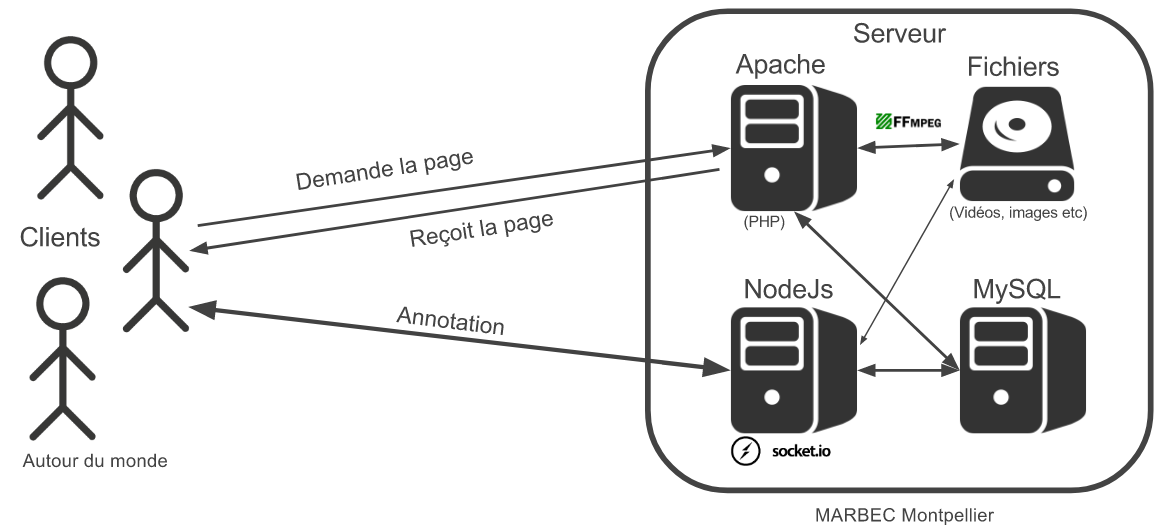
\includegraphics[width=1\textwidth]{img/oia_v1_schema.png}
 \caption{Schema des liaisons OIA V1}
 %\label{fig:schema_liaison_v1}
\end{figure}

Le serveur Node.js sert de passerelle pour les annotations et utilise les Web socket pour créer un flux tendu entre le client et le serveur. L’information transite sous forme de texte JSON, facilement interprétable en JavaScript côté client et côté serveur. Pour simplifier l’utilisation des Web socket le package socket.IO est utilisé.
[Figure 2]
\newpage
\begin{figure}[H]
\centering
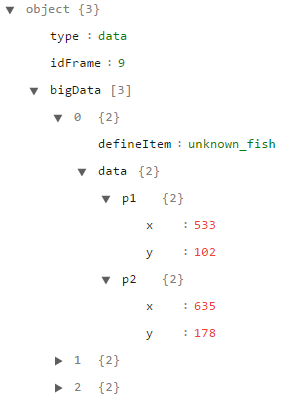
\includegraphics[width=0.5\textwidth]{img/infoFrameData.png}
 \caption{Données passées dans les WebSockets}
 \label{fig:donnee_websockets}
\end{figure}
Node.js est une plateforme logiciel libre et événementielle en JavaScript. Basée sur le Moteur JS V8 de google, il fonctionne sur un principe de code non bloquant, laissant ainsi plusieurs parties de code s'exécuter en même temps. Ces principes de code non bloquant de programmation événementielle offre à l'application d'annotation vitesse et stabilité.

\par
Pour le découpage des vidéos et l’extraction des images, le logiciel ffmepg est utilisé. Il permet d’extraire des images à intervalles réguliers tout au long de la vidéo. Il est donc possible d’extraire entre 0 et plus de 25 images par seconde et ainsi créer un « projet » contenant les images et le fichier d’informations :

\begin{itemize}
    \item Le nom du projet.
    \item Le nom de la vidéo.
    \item La fréquence d’extraction.
    \item Le nombre d’images extraites.
    \item Test utilisateur ou non.
    \item Le nom de l’utilisateur si le projet est un test.
\end{itemize}
Un projet est un dossier contenu dans le même dossier que sa vidéo et est facilement déplaçable ailleurs.
\par
La base de données SQL est utilisée pour la gestion des utilisateurs, des données vidéos et projets ainsi que de la liste des objets (famille, genus, espèce). [Figure 3]

\begin{figure}[H]
\centering
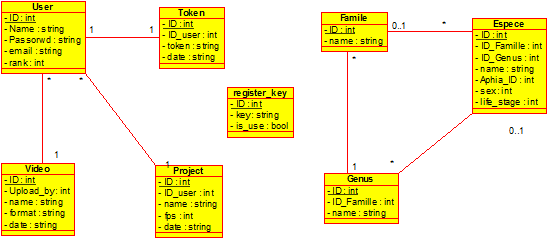
\includegraphics[width=1\textwidth]{img/class_diagram_V1.png}
 \caption{Base de données SQL}
 \label{fig:BDD_SQL_V1}
\end{figure}

Un utilisateur ne peut s’inscrire que par l’utilisation d’une clé unique générée par un administrateur.
Ces clés sont à utilisation unique.

Les limites de la solution actuelle sont la validation et le traitement des données. En effet, les fichiers JSON sont partagés pour un fichier par image dans chaque projet. Ce système limite la lecture des données à une lecture locale peu rapide.
\par
Exemple :
\par
\begin{itemize}
    \item Un projet peut contenir plus de 6000 images et donc 6000 fichiers JSON. Il faudrait lire tous les fichiers de chaque projet ce qui représente une quantité de fichiers conséquentes dans l’optimisation de la vitesse et l’accès aux données.
    \item La traçabilité des données pour les annotations des utilisateurs.
    \item La liste des objets est limitée à trois colonnes : famille, genus, espèce.
    \item Trop spécialisé.
\end{itemize}


\section{Nouvelle version}
Cette nouvelle version intègre une nouvelle base de données NoSQL : MongoDB
La base mongodb remplace le système de fichiers JSON ainsi qu’une partie de la base SQL. [Figure 4]

\begin{figure}[H]
\centering
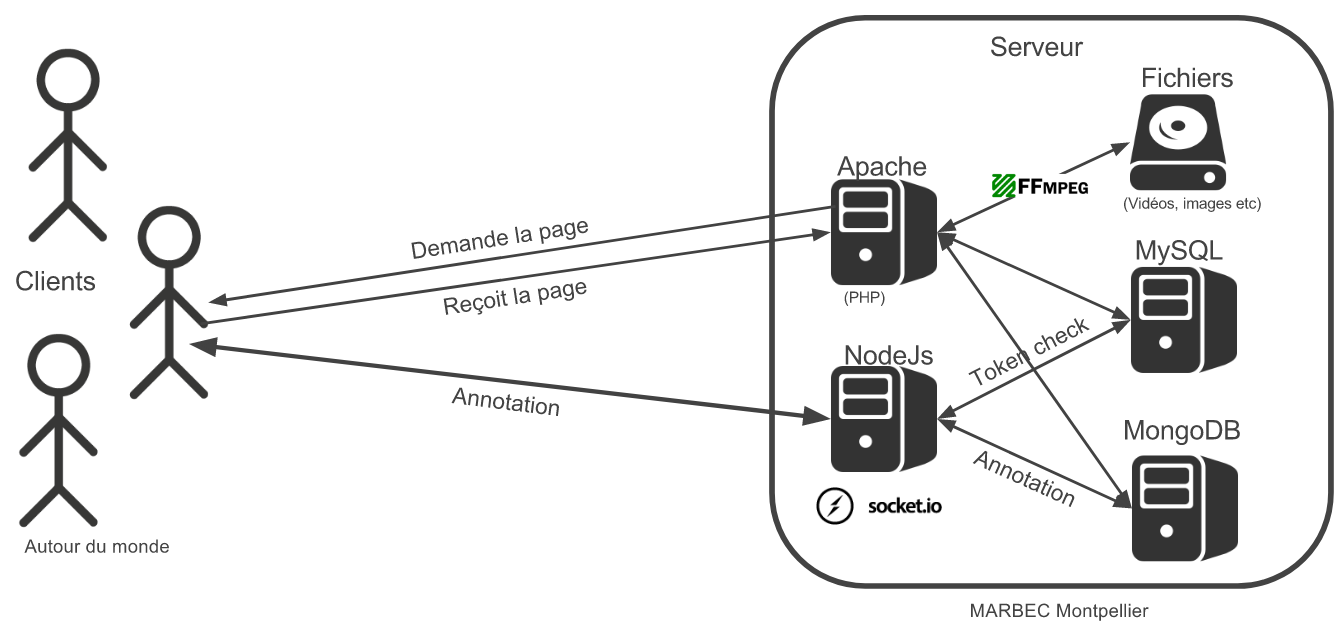
\includegraphics[width=1\textwidth]{img/oia_v2_schema.png}
 \caption{Schema des liaisons OIA V2}
 \label{fig:schema_liaison_v2}
\end{figure}

Mongodb est un système de gestion de base de données NoSQL basées sur du JSON (BSON : Binary JSON). Faite pour traiter de très grosses quantités de données, mongodb offre la souplesse et les capacités de traitement qui faisait défaut à l’ancien système de fichiers JSON utilisé.
\par
Il devient aussi possible de déporter cette base de données sur un autre serveur et ainsi séparer les services.
\par
Le langage R utilisé par les biologistes possède des packages ajoutant des possibilités d’interaction avec ce type de base de données (mongodb). Ainsi il est possible d’interroger en direct sans exportation de données, la base d’annotation.

\begin{figure}[H]
\centering
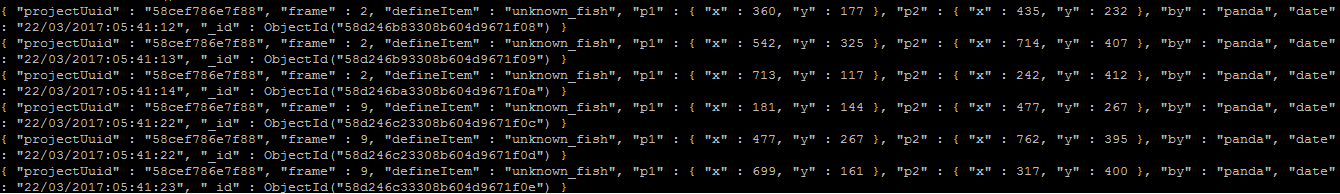
\includegraphics[width=1\textwidth]{img/OIA_V2/oia_v2_05.png}
 \caption{Extrait de la collection d'annotation}
 \label{fig:collection_anno}
\end{figure}

\par
En changeant de système d’enregistrement des données vidéo par mongodb, l’ajout après upload et avant création de projet, des informations sur la vidéo (position GPS, de prise, profondeur etc.) se fait de manière simple et sans contrainte.

\begin{figure}[H]
\centering
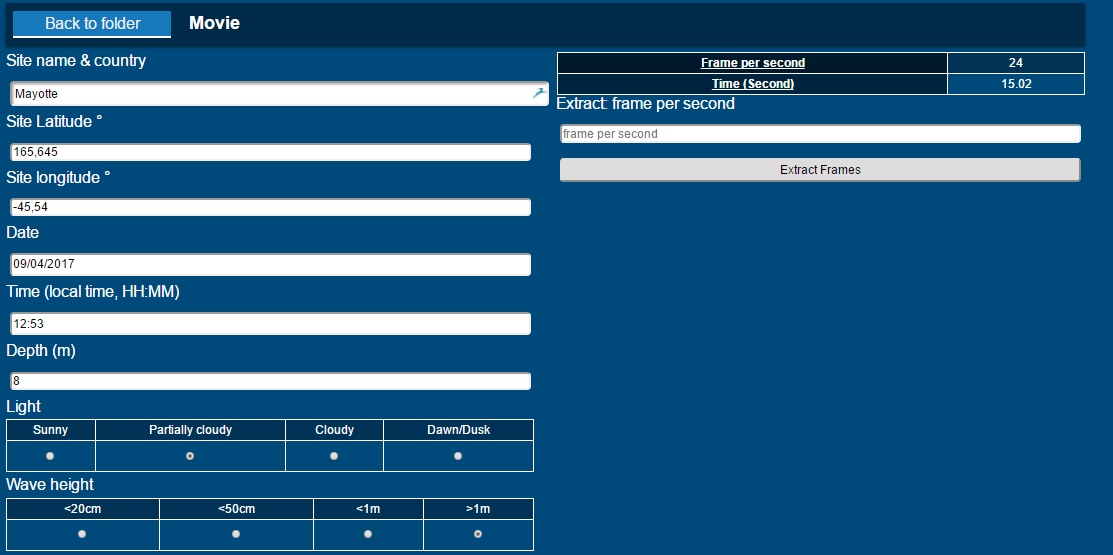
\includegraphics[width=1\textwidth]{img/OIA_V2/oia_v2_08.png}
 \caption{Interface des données vidéo}
 \label{fig:donnee_video}
\end{figure}

\par
L’ajout d’une barre de recherche dans la liste des espèces devenait indispensable au vu de la quantité d’objets enregistrés (plus de 350) ce fut donc aussi un des ajouts intégrés dans cette version.
\begin{figure}[H]
\centering
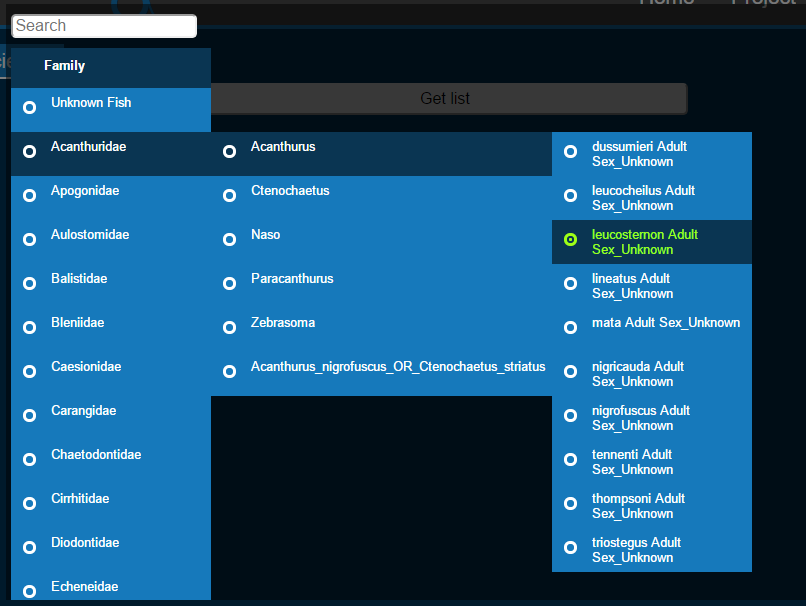
\includegraphics[width=1\textwidth]{img/OIA_V1/oia_v1_04.png}
 \caption{Bare de recherche}
 \label{fig:donnee_video}
\end{figure}
\begin{figure}[H]
\centering
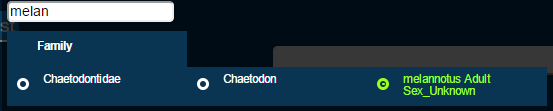
\includegraphics[width=1\textwidth]{img/OIA_V2/oia_v2_09.png}
 \caption{Barre de recherche}
 \label{fig:donnee_video}
\end{figure}

Plus d’informations et de lisibilité au niveau de la navigation fichiers.
Les fonds verts indiquent des projets dits de « vérité » les fonds orange indiquent seulement les projets de test avec annotations individuelles.

\begin{figure}[H]
\centering
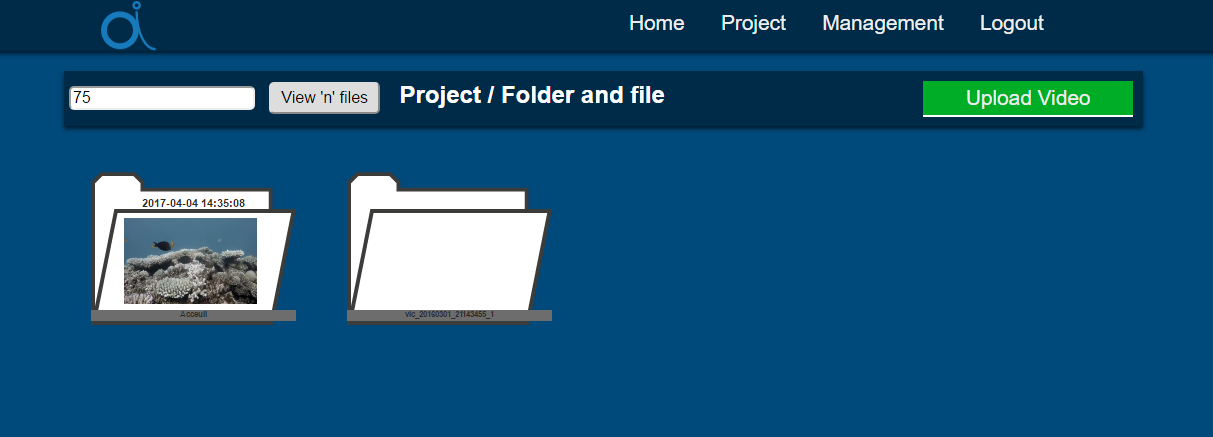
\includegraphics[width=1\textwidth]{img/OIA_V2/oia_v2_02.png}
 \caption{Navigation fichier}
 \label{fig:nav_1}
\end{figure}
\begin{figure}[H]
\centering
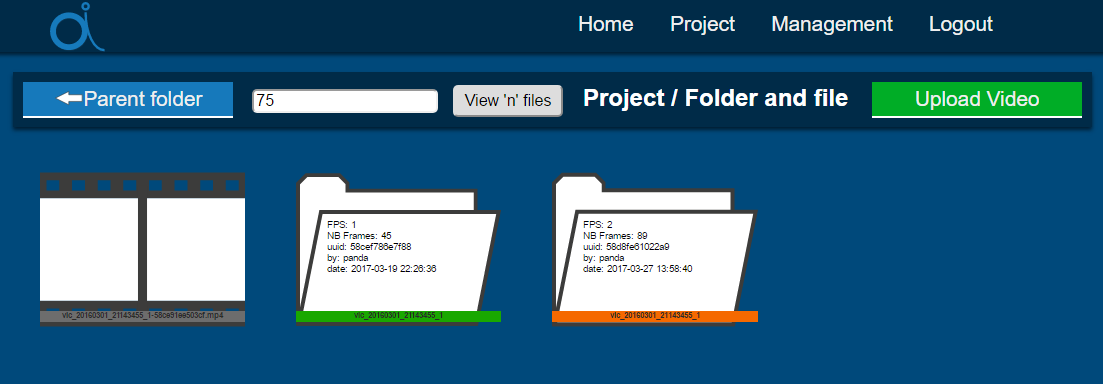
\includegraphics[width=1\textwidth]{img/OIA_V2/oia_v2_03.png}
 \caption{Navigation fichier}
 \label{fig:nav_2}
\end{figure}

Comparatif des versions :

\begin{figure}[H]
\centering
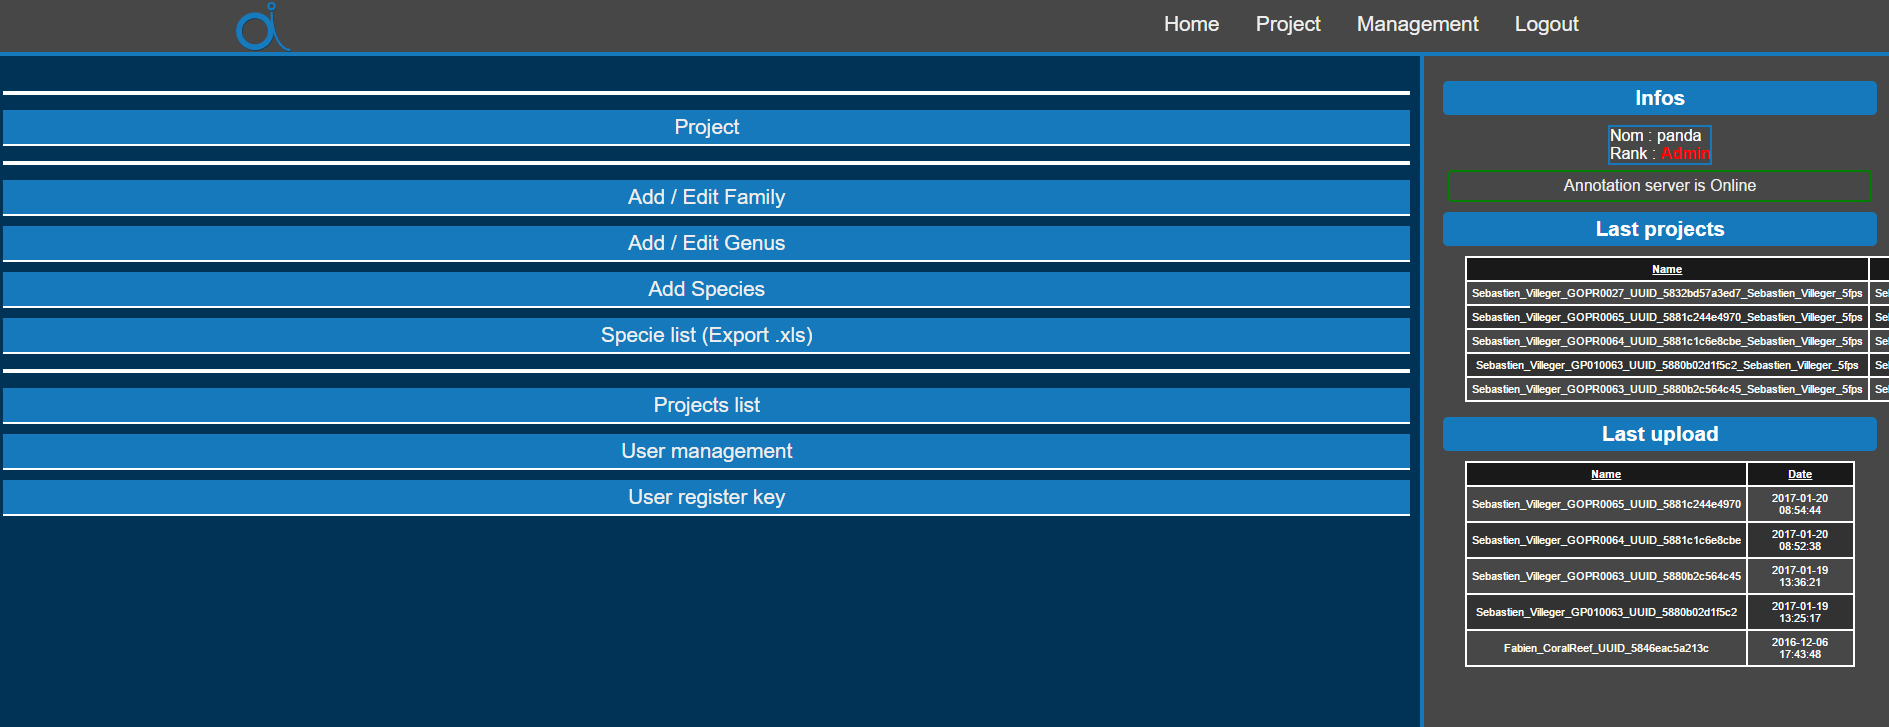
\includegraphics[width=1\textwidth]{img/OIA_V1/oia_v1_01.png}
 \caption{Menu OIA V1}
 \label{fig:menu_v1}
\end{figure}
\begin{figure}[H]
\centering
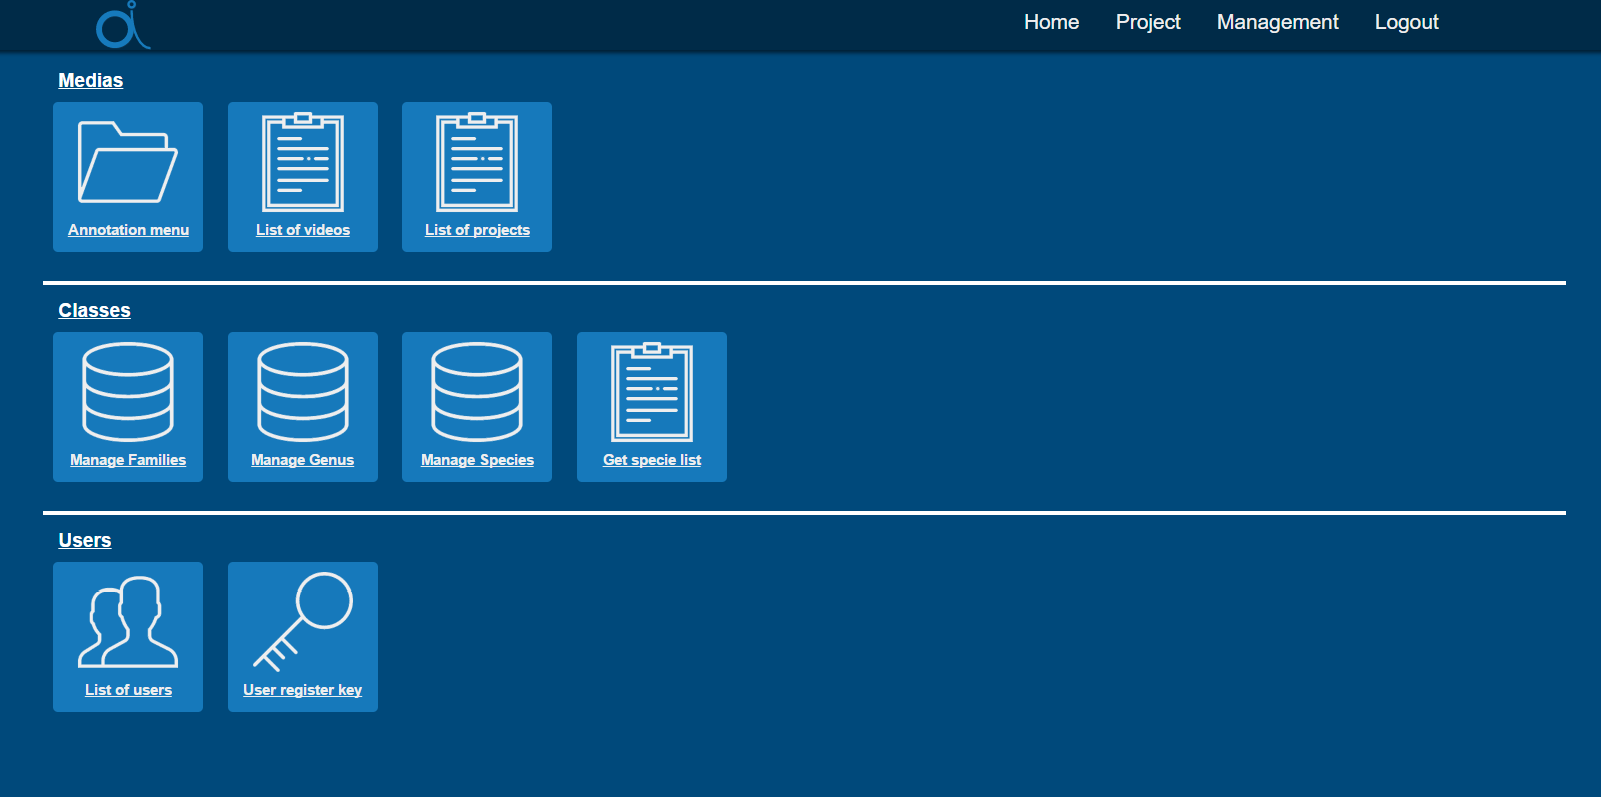
\includegraphics[width=1\textwidth]{img/OIA_V2/oia_v2_01.png}
 \caption{Menu OIA V2}
 \label{fig:menu_v2}
\end{figure}

Meilleure séparation des parties. Images en SVG pour responsive design.
(Optimisation de l'affichage selon les formats d'écran)

\begin{figure}[H]
\centering
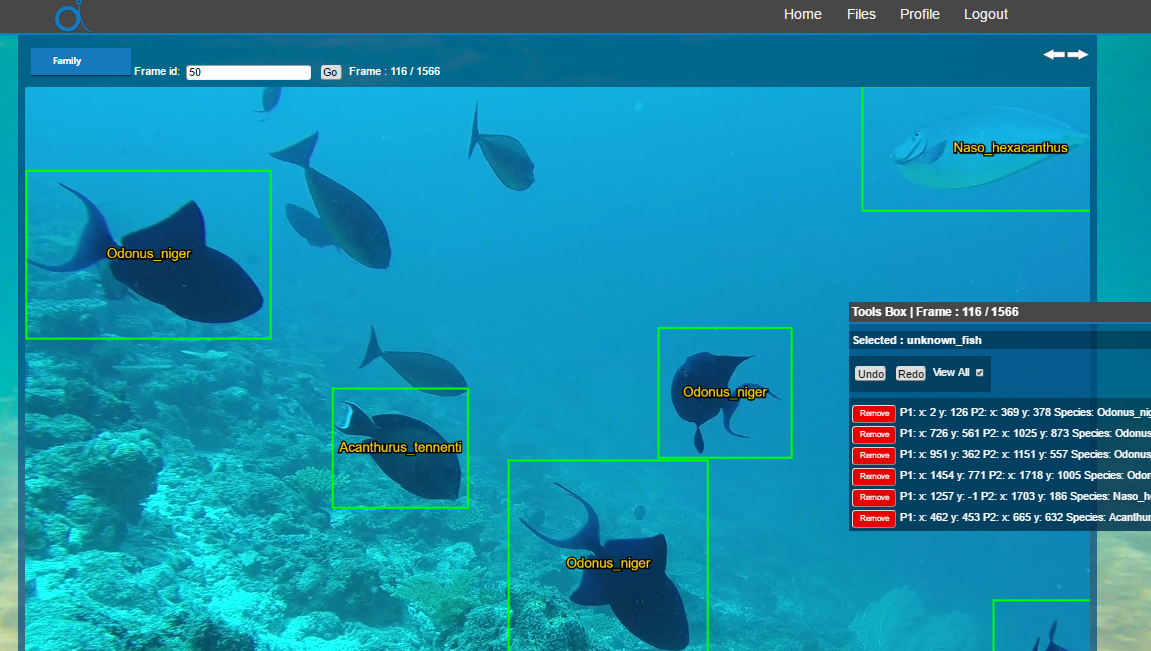
\includegraphics[width=1\textwidth]{img/OIA_V1/oia_v1_06.png}
 \caption{Interface d'annotation V1}
 \label{fig:anno_v1}
\end{figure}
\begin{figure}[H]
\centering
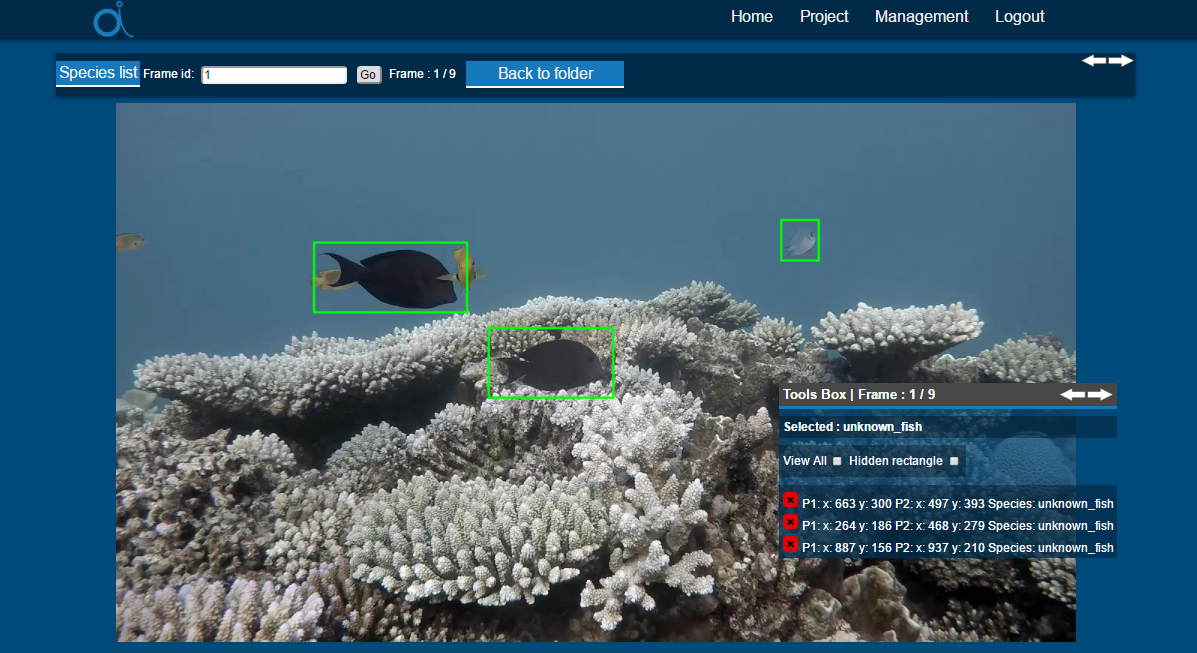
\includegraphics[width=1\textwidth]{img/OIA_V2/oia_v2_07.png}
 \caption{Interface d'annotation V2}
 \label{fig:anno_v2}
\end{figure}

Suppression de la limite par un cadre de la taille de l'image (Limite les scrollbars).
Diminution des boutons de suppression pour limiter la taille de la "tools box".
Tools box plus simple à déplacer sur la fenêtre. Liste des objets affichée dans une sur-fenêtre.

\newpage

\section{Méthodologie de travail}

Plusieurs personnes sont en relation avec ce projet.
\par
Monsieur Pompidor, encadrant du TER pour l'Université. Il apporte son aide côté technique par ses connaissances sur MongoDB et NodeJS. Il aide dans l’aiguillage des réalisations en cours.
\par
Sébastien Villeger encadrant laboratoire MARBEC pour qui l’application a été créée. Il définit les besoins et les priorités pour l’application.
\par
Sébastien Villon, personne en charge du Deep Learning. Les exigences d’annotation, d’exportation et de définition des objets ont été fournies par lui.
\par
Une réunion en moyenne toutes les une ou deux semaines selon la disponibilité de chacun est organisée, avec l’encadrant du TER pour faire un point sur l’avancement et les problèmes rencontrés sur le projet. De plus une visite régulière au laboratoire MARBEC compléte les besoins d’information.
\par
Un dépôt GIT est utilisé pour la gestion des versions, un cloud a été mis en oeuvre pour synchroniser des documents ou des vidéos d’essai et limiter les pertes en cas de mauvaise manipulation ou de problèmes informatiques.

\begin{figure}[H]
\centering
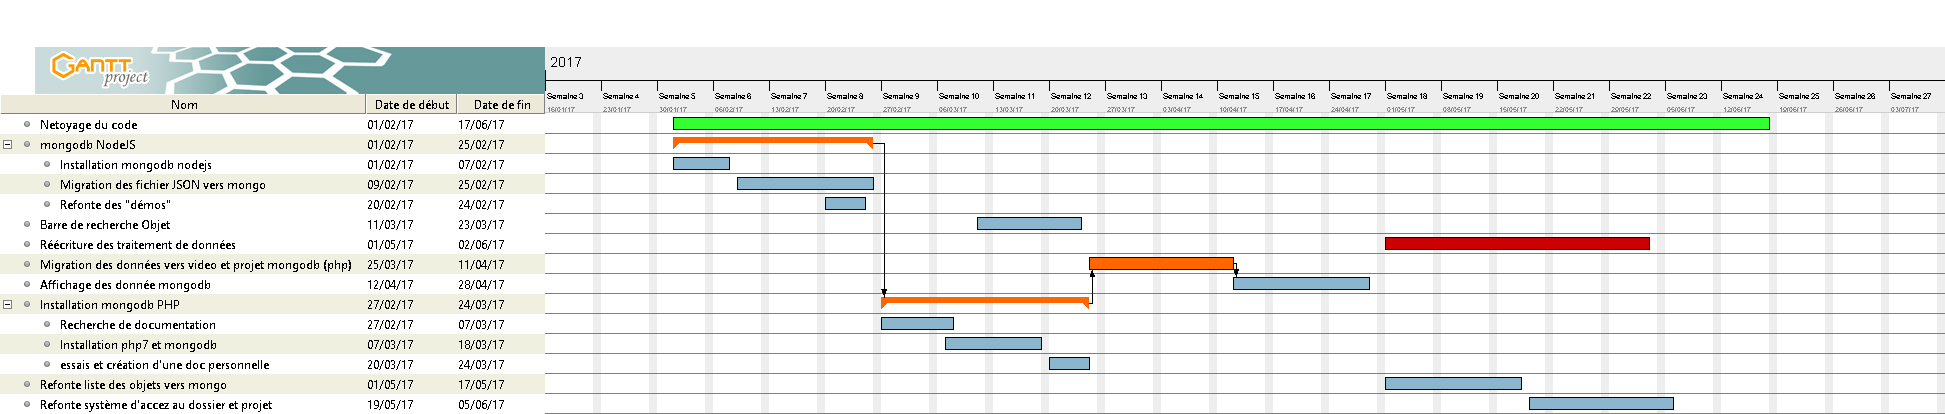
\includegraphics[width=1\textwidth]{img/gantt_oia.png}
 \caption{Diagramme de Gantt}
 \label{fig:gantt}
\end{figure}


\section{Réalisation}
La plus grosse partie du projet consistait à migrer les données MongoDB. Cette migration demandait la refonte totale de la partie traitement des annotations du serveur NodeJS. Sur l’ancienne version le serveur demandait la position du projet dans l’arborescence de fichiers pour écrire les fichiers JSON dans le dossier projet. Il a donc fallu remplacer ce système par un système d’identifiant unique raccordé au projet. De plus les projets dits de tests ont leurs annotations dans une autre collection afin d’éviter les conflits avec les annotations ; de vérifier les annotations utilisées pour le deep Learning ou autre. De même que la lecture des informations d’un projet qui se situait dans un fichier nommé « informations.json » ont aussi été déplacées sur la base NoSQL et devaient aussi être accordées avec le serveur NodeJS.
\par
Ces changements ont permi la découverte et la correction de bogues qui nuisaient au confort d’utilisation ; comme des problèmes d’asynchronisation ou de crash serveur.
Par exemple à partir d’un certain nombre d’utilisation la fonction d’annulation provoquait des crash serveur. Le retrait temporaire de cette fonction avant refonte ne gêne pas l’utilisation de l’application car il est toujours possible de supprimer ce que l’on vient de faire et de le refaire.
\par
Une seconde part importante de ce projet fut donc la correction et l’optimisation du code existant par de nouveaux algorithmes plus rapides et moins hasardeux au niveau de l’asynchronisme pour NodeJS. Ces changements demandaient aussi à être faits sur le serveur Apache avec PHP.
\par
Le développement et l’insertion de nouvelles fonctionnalités fut soit simple et ne demandait pas de changement dans le code existant mais pouvait demander un temps de développement assez large, soit très simple à développer mais un remodelage de certaines parties du code pouvait être fait.

\newpage

\section{Conclusion}
A ce jour la nouvelle version de l’application est sur un serveur de test avec la majeure partie des nouveaux besoins et changements effectués. La partie annotations est entièrement utilisable que ce soit pour les annotations deep Learning ou de test, la sauvegarde des données vidéo fonctionne et les corrections dans l’ergonomie et des plus gros bugs ont été faites. Il ne reste plus que l’exportation des données à terminer mais cette fonction peut être faite après la phase de déploiement sur le serveur utilisée par l’ancienne version.
\par
En perspective, il est prévu de changer le système de liste d’objets par un système d’arbres génériques non plus en SQL mais sur la base MongoDB ; ainsi que quelques changements dans l’affichage et la navigation dans les fichiers.
Le futur système de liste d’objets possède déjà une structure de sa base de données et les changements qui vont avec ont déjà été listés.
\par
De manière personnelle ce projet m’a permis de découvrir et manipuler d’autres types de bases de données que des bases SQL. De nouvelles connaissances en PHP, en JS, en optimisation et correction de code. La communication entre différents types de domaine avec la convergence nécessaire sur le vocabulaire utilisé, ou les reformulations des idées, m'a fait beaucoup progresser et m'a apporté une certaine agilité d'esprit.


%\newpage

%\section{Annexes}

%Rapport Stage :\par
%https://drive.google.com/open?id=0B0URPqXwXxBURXBQLTgxYXc2ZE0

%Document d'installation personnel après recherche :\par
%https://drive.google.com/open?id=0B0URPqXwXxBUaUxQMmxCb05YSFE



%\bibliographystyle{plain}
%\bibliography{references}
\end{document}
